\subsection{ECTS}
\label{SubsectionECTS}
The idea of eTSC evolved over time. In the beginning, similar concepts to eTSC existed where the main goal was to classify prefixes of data, but these techniques
lacked the reasoning of how to provide reliable classification results\cite{lv2019effective,santos2016literature}.
One of the earliest papers that formally defined eTSC as a tradeoff between earliness and accuracy was the paper by \cite{xing2009early}, proposing a technique which is named after the problem itself; Early Time Series Classification (ECTS).
The main idea was to examine the stability of of Nearest Neighbor approaches, to keep correctly classifying data instances, in the space of full length series and the subspaces created from subsequences of the training data set \cite{lv2019effective,mori2017early}.
ECTS utilizes the concept of reverse nearest neighbors (RNN) to learn for each training instance the Minimum Prediction Length (MPL).
MPL represents the earliest point in time for which a training instance can be used to classify a query instance without loss of accuracy.
The definition mentioned by \cite{xing2009early} defines MPL as:
\begin{definition}
    In a training data set $T$ with full-length $L$, for a time series $t \epsilon T$,
    the minimum prediction length (MPL for short) of $t$, $MPL(t) = k$
    if for any $l(k \leq l \leq L)$, (1) $RNN\textsuperscript{l}(t)$ = $RNN\textsuperscript{L}(t) \neq \varnothing$ and (2) $RNN\textsuperscript{k−1}(t) \neq RNN\textsuperscript{L}(t)$.
    Specifically, if $RNN\textsuperscript{L}(t) = \varnothing$, then $MPL(t) = L.$
\end{definition}
During classification MPL is calculated for each instance (in the same study a relaxed variant is introduced using clusters of instances).
As for the classification, as the data points of the testing instance start to arrive, the classification method tries to find the nearest instance which has reached it's MPL.
If there was no suh instance found, then more data points are needed till a trusted classification can be done.
ECTS was criticized \cite{he2015early,ghalwash2014utilizing,xing2011extracting} because it is based on nearest neighbor approaches; which only provide classification results based on distance
without deriving patterns from the data. This means that data users cannot attain insights about the problem using the results.

\subsection{Shapelet Based Algorithms}
\label{SubsectionETSCAShapelets}
A group of methods \cite{xing2011extracting,ghalwash2012early,ghalwash2014utilizing,he2015early} focused on the interpretability of the results obtained by eTSCAs,
motivated by domains where not only correct classification is important, but also getting insights and understanding what contributed to the final result.
One of these domains would be the medical field, where undesrtanding the reason for a patient's disease is very important than just linking the patient to previously seen patients \cite{xing2011extracting}.
Shapelets provided a good solution for these methods. Since shapelets, as previously mentioned, are defined as unique subsequences which can uniquely identify classes.
Early Distinctive Shapelet Classification (EDSC) was a framework consisting of 2 steps; feature extraction and feature seletion.
In the feature extraction step, all local shapelets are extracted and a distance threshold is learned. EDSC developed a technique which they called the best-matching-distance (BMD),
which consideres a shapelet to be distinctive, by comparing it to all instances in the training data set and considering target classes distribution.
If the majority of instances closer to the shapelet belong to a target class, it is considered to be distinctive of this class.
In the feature selection step, EDSC selects a smaller set of features based on three main criteria; earliness, frequency and distinctivness.
EDSC was later extended in two different directions.

In \cite{ghalwash2012early} EDSC was extended in the aspect of data dimensionality; as the original EDSC only convered univariate data sets.
The extension covered; adapting the feature extraction to discover multivariate shapelets along with calculating distance thresholds for each dimension and
using a distance threshold based on information gain, adapting the feature selection step, by modifying the equations calculating the notions of earliness, frequency and distinctivness to multiple dimensions.
In \cite{ghalwash2014utilizing} EDSC was extended in the aspect of data uncertainty. The main idea was that shapelets use a distance threshold when being compared to instances,
if the distance between the shapelet and the instance is less than the threshold, the instance is given the label of the shapelet.
On the other hand, since the threshold represents a range, a shapelet is more certain of the class label given to an instance which has a distance closer to 0 than the class label given to an instance falling on the limits of the threshold.
Motivated by the interest of uncertainty in the medical field, the goal was to provide a notion of uncertainty along with the interpretability of shapelets.
The proposed Modified EDSC with Uncertainty estimates (MEDSC-U) calculated uncertainty as (1 - confidence), where confidence is a numeric value represting two aspects;
confidence that the distance between the shapelet and the instance is less than the threshold and confidence that the shapelet can correctly classify the instance.
This confidence notion could then be generalized for classes represented by multiple shapelets.
The issue of confidence for eTSC had been discussed in other papers like \cite{parrish2013classifying} and \cite{lv2019effective}.

\subsection{ECDIRE}
\label{SubsectionECDIRE}
The paper by \cite{mori2017reliable} propsed a new framework; Early Classification of Time Series based on Discriminating Classes Over Time (ECDIRE).
There were two goals that ECDIRE wanted to achieve \cite{mori2017early}.
The main goal of the framework was to track the accuracy evolution for a group of probabilistic classifiers across time; to identify safe time points after which
predictions can be made. This would allow for avoiding unnecessary checking at each time point. The other goal was to offer an outliers discarding mechanism using a reliability condition.
ECDIRE consisted of three training steps. In the first step the framework analyzes the data set and tries to identify the safe points at which classes can be differentiated from each other.
This is done by defining time points as percentages of the full length and training, at each time point, a probabilistic classifier.
The early points are then defined as those which maintain an accuracy of a desired percentage from that obtained on the complete data \cite{santos2016literature}.
In the second step, a reliability threshold is determined using the class probabilities of the assigned class and the second highest class;
this helps avoid uncertain classifications or very soon time points. In the last step, the final probabilistic classifiers are trained using the early time points
identified in the first step. As a backup plan, if the last early time point did not coincide with the full length of the time series, ECDIRE acts like other methods and
builds classifiers on each time point.

\subsection{TEASER}
\label{SubsectionTEASER}
One of the latest classifiers introduced is the Two-tier Early and Accurate Series classifiER (TEASER) \cite{schafer2020teaser}.
TEASER's main focus was challenging the logic of previous classifiers on determining the point of time at which a classification can be assigned to a time series instance.
Previous methods would try to learn from the training data set a fixed prefix needed to be seen before it can start classification; like MPL in ECTS and EDSC, or to learn a safe point like in ECDIRE.
These techniques would require the classifiers to always wait till they reach these fixed points of time before they can assign a label.
Whereas TEASER was designed to give a classification once confident of it's decision, and not to depend on any fixed time points nor assume that all data instances were recorded
at the same starting point.
TEASER models the problem of eTSC with a two tier solution. In the first tier, a slave classifier is regularly checking the incoming data and assigning class probabilities.
These probabilities are then assessed in the second tier by a master classifier, which either accepts the classification from the slave, or rejects it and decides to wait for more data to arrive.
The classifiers are paired through out the whole process, such that for each slave classifier there is a master classifier that reads it's output and assesses it's results.
TEASER starts off by defining the number of classifier pairs that will be neeeded, this is calculated by dividing the length of the longest data instance in the training data set
by the window length which is a user defined parameter. Which is noted as $S = [n_{max}/w]$, where $n_{max}$ is the length of the longest instance and w is the window length.
During training, slave classifiers are trained on subsequences $s_{i}$, or snapshots, of the time series where the length of $s_{i} = i . w $. These snapshots are z-normalized based on
the values existing only in them and not on values from the full length data as recommended by \cite{mori2017early}.

The slave classifiers would then calculate three features; the class label with the highest probability $c(s_{i})$, the vector of class probabilities for all available classes $P(s_{i})$,
and the difference between the class probability of the highest two classes denoted as $\Delta d$.
These three features are then passed to the paired master classifier, which trains a model over them using a one-class Support Vector Machine (oc-SVM).
A parameter that plays an important role in this process is $v$, it is the number of consecutive times the same class label is given to an instance.
Once the same label is given $v$ times for consecutive snapshots, the master classifier is confident of this class label.
Figure \ref{Img:TEASER} shows an example of how TEASER components handle a misleading data instance from the traces of microwave and a digital receiver.

\begin{figure}
    \captionsetup{justification=raggedright}
    \centering
    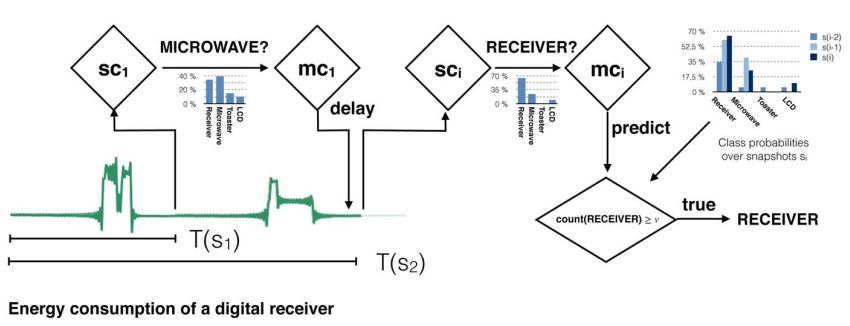
\includegraphics[scale = 0.65]{TEASER.JPG}
    \centering
    \caption{TEASER is given a snapshot of an energy consumption time series. After seeing the first s measurements, the first slave classifier $sc_{1}$ performs a prediction which the master classifier $mc_{1}$ rejects due to low class probabilities. After observing the i-th interval which includes a characteristic energy burst, the slave classifier $sc_{i}$ (correctly) predicts RECEIVER, and the master classifier $mc_{i}$ eventually accepts this prediction. When the prediction of RECEIVER has been consistently derived v times, it is output as final prediction  \cite{schafer2020teaser}}
    \label{Img:TEASER}
\end{figure}